\newpage

\section{Annexes}

\begin{figure}[H]
  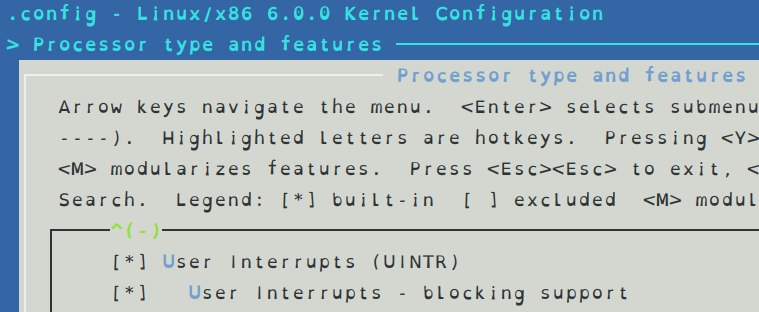
\includegraphics[width=\textwidth]{enableFeaturesInConfigMenu}
  \caption{Activé le support des uintr à la compilation du noyau}
  \label{fig:enableFeaturesInConfigMenu}
\end{figure}

\begin{figure}[H]
  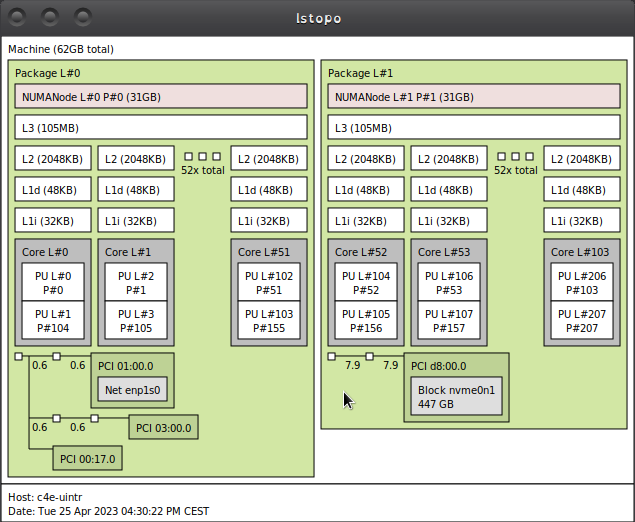
\includegraphics[width=\textwidth]{lstopoC4eUintr}
  \caption{Topologie de la machine fourni par \emph{Atos} obtenus grâce à la command \emph{lstopo}}
  \label{fig:lstopo}
\end{figure}

\begin{figure}[H]
  \begin{subfigure}{\textwidth}
    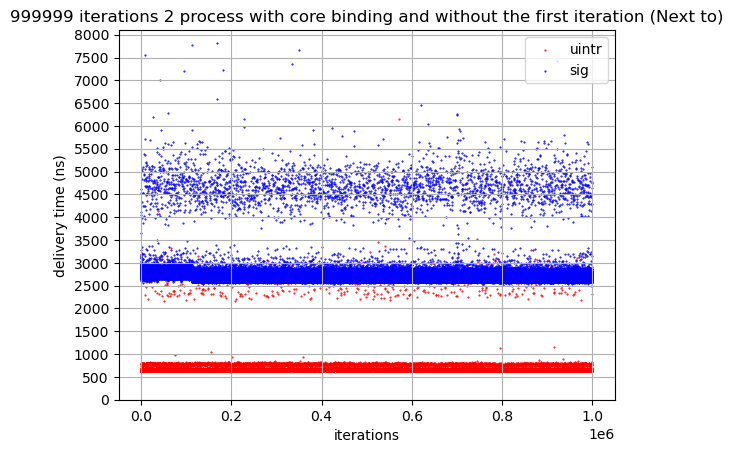
\includegraphics[width=\textwidth]{latency/1e6ProcessNT}
    \caption{}
    \label{subfig:latency1e6ProcessNT}
  \end{subfigure}
  \begin{subtable}{\textwidth}
    \centering
    \begin{tabular}{| l | l | l | l | l | l | l | l |}
      \hline
      &\bf mean &\bf std &\bf min  &\bf 10\% &\bf 50\% &\bf 95\% &\bf max\\
      \hline
      \bf sig   & 2675 & 147 & 2520 & 2620 & 2658 & 2781 & 44311\\
      \hline
      \bf uintr & 651  & 72  & 631  & 642  & 649  & 659  & 46053\\
      \hline
    \end{tabular}
    \caption{}
    \label{tab:latency1e6ProcessNT}
  \end{subtable}
  \caption{Mesures de latence entre deux process avec un placement proche}
  \label{fig:latency1e6ProcessNT}
\end{figure}

\begin{figure}[H]
  \begin{subfigure}{\textwidth}
    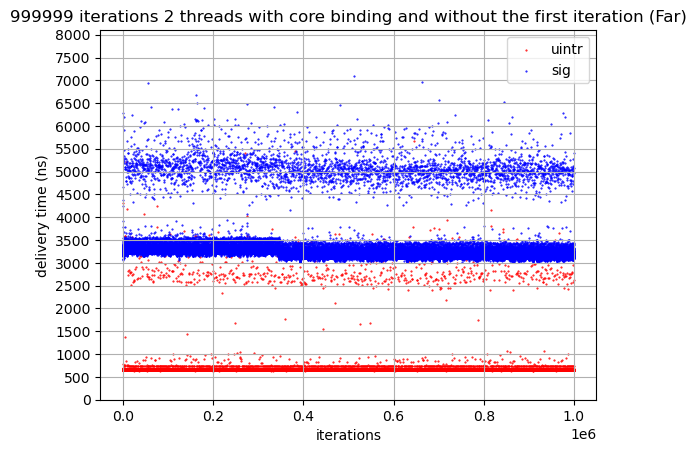
\includegraphics[width=\textwidth]{latency/1e6ThreadsF}
    \caption{}
    \label{subfig:latency1e6ThreadsF}
  \end{subfigure}
  \begin{subtable}{\textwidth}
    \centering
    \begin{tabular}{| l | l | l | l | l | l | l | l |}
      \hline
      &\bf mean &\bf std &\bf min  &\bf 10\% &\bf 50\% &\bf 95\% &\bf max\\
      \hline
      \bf sig   & 3210 & 156 & 3014 & 3141 & 3177 & 3302 & 63690\\
      \hline
      \bf uintr & 654  & 329 & 638  & 648  & 653  & 659  & 325408\\
      \hline
    \end{tabular}
    \caption{}
    \label{tab:latency1e6ThreadsF}
  \end{subtable}
  \caption{Mesures de latence entre deux threads avec un placement éloigné}
  \label{fig:latency1e6ThreadsF}
\end{figure}

\begin{figure}[H]
  \begin{subfigure}{\textwidth}
    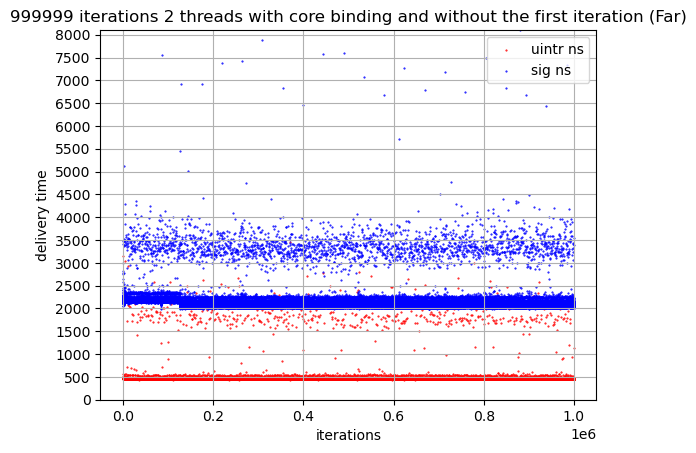
\includegraphics[width=\textwidth]{latency/1e6ThreadsF_TB}
    \caption{}
    \label{subfig:latency1e6ThreadsF-TB}
  \end{subfigure}
  \begin{subtable}{\textwidth}
    \centering
    \begin{tabular}{| l | l | l | l | l | l | l | l |}
      \hline
      &\bf mean &\bf std &\bf min  &\bf 10\% &\bf 50\% &\bf 95\% &\bf max\\
      \hline
      \bf sig   & 2097 & 282 & 1981 & 2064 & 2082 & 2178 & 270625\\
      \hline
      \bf uintr & 455  & 389 & 440  & 450 & 454 & 460 & 388815\\
      \hline
    \end{tabular}
    \caption{}
    \label{tab:latency1e6ThreadsF-TB}
  \end{subtable}
  \caption{Mesures de latence entre deux threads avec un placement éloigné et le turbo boost activé}
  \label{fig:latency1e6ThreadsF-TB}
\end{figure}

\begin{figure}[H]
  \begin{subfigure}{\textwidth}
    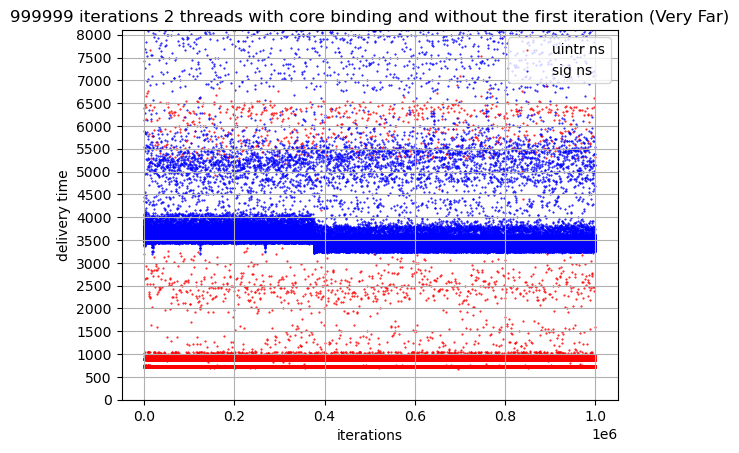
\includegraphics[width=\textwidth]{latency/1e6ThreadsVF_TB}
    \caption{}
    \label{subfig:latency1e6ThreadsVF-TB}
  \end{subfigure}
  \begin{subtable}{\textwidth}
    \centering
    \begin{tabular}{| l | l | l | l | l | l | l | l |}
      \hline
      &\bf mean &\bf std &\bf min  &\bf 10\% &\bf 50\% &\bf 95\% &\bf max\\
      \hline
      \bf sig   & 3520 & 327 & 3189 & 3383 & 3481 & 3678 & 51798\\
      \hline
      \bf uintr & 736  & 159 & 683 & 721 & 725 & 735 & 46787\\
      \hline
    \end{tabular}
    \caption{}
    \label{tab:latency1e6ThreadsVF-TB}
  \end{subtable}
  \caption{Mesures de latence entre deux threads avec un placement très éloigné et le turbo boost activé}
  \label{fig:latency1e6ThreadsVF-TB}
\end{figure}
